\documentclass[
    floatfix, aps, pra, superscriptaddress,
	10pt, twocolumn,
    % noshowpacs,
	% floatfix,nobibnotes,
    nofootinbib,
	tightenlines
]{revtex4-1}
%\pdfoutput=1

\usepackage{graphicx}
\usepackage{amsmath,soul,mathtools}
\usepackage{amssymb}
% \usepackage{times}
\usepackage{bbm}
\usepackage{bm}
\usepackage[T1]{fontenc}
\usepackage{bbold}
% \usepackage{nccmath}
\usepackage[mathscr]{eucal}
% \usepackage{multirow}
\usepackage{colortbl}
\usepackage{listings}
\usepackage[utf8]{inputenc}
\usepackage{lmodern}
\usepackage[caption=false]{subfig}

% \usepackage{ifthen}
\usepackage{booktabs}
\usepackage{tabularx}

\usepackage{hyperref}
\hypersetup{
    colorlinks = true
}
\usepackage{cleveref}
\usepackage{array}
\usepackage{soul}
\usepackage{easyReview}
\usepackage{physics}
\usepackage{siunitx}

\usepackage{acronym}
\newacro{ML}{Machine Learning}
\newacro{VVB}{Vector Vortex Beam}
\newacro{QW}{Quantum Walk}
\newacro{CNN}{Convolutional Neural Network}
\newacro{ANN}{Artificial Neural Network}
\newacro{LG}{Laguerre-Gauss}
\newacro{HG}{Hermite-Gauss}
\newacro{OAM}{Orbital Angular Momentum}
\newacro{SAM}{Spin Angular Momentum}
\newacro{CCD}{Charged-Coupled Device}
\newacro{SVM}{Support Vector Machine}
\newacro{DR}{Dimensionality Reduction}
\newacro{PCA}{Principal Component Analysis}
\newacro{RBF}{Radial Basis Function}

\newcommand{\bs}[1]{\boldsymbol{#1}}
\newcommand{\on}[1]{\operatorname{#1}}
\newcommand{\RR}{\mathbb{R}}

\newcommand{\addrm}[1]{{\color{purple}{#1}}}
% \newcommand{\remove}[1]{{\color{orange}\st{#1}}}
% \newcommand{\add}[1]{{\color{blue}{#1}}}
\newcommand{\rmv}[1]{{\color{red}\st{#1}}}
\newcommand{\redComm}[1]{\textcolor{red}{\small[#1]}}

\begin{document}
\title{Supplemental material: Machine learning-based classification of vector vortex beams} 
\author{Taira Giordani}
\affiliation{Dipartimento di Fisica, Sapienza Universit\`{a} di Roma,
Piazzale Aldo Moro 5, I-00185 Roma, Italy}

\author{Alessia Suprano}
\affiliation{Dipartimento di Fisica, Sapienza Universit\`{a} di Roma,
Piazzale Aldo Moro 5, I-00185 Roma, Italy}

\author{Emanuele Polino}
\affiliation{Dipartimento di Fisica, Sapienza Universit\`{a} di Roma,
Piazzale Aldo Moro 5, I-00185 Roma, Italy}
\author{Francesca Acanfora}
\affiliation{Dipartimento di Fisica, Sapienza Universit\`{a} di Roma,
Piazzale Aldo Moro 5, I-00185 Roma, Italy}


\author{Luca Innocenti}
\affiliation{Centre for Theoretical Atomic, Molecular, and Optical Physics,
School of Mathematics and Physics, Queen's University Belfast, BT7 1NN Belfast, United Kingdom}


\author{Alessandro Ferraro}
\affiliation{Centre for Theoretical Atomic, Molecular, and Optical Physics,
School of Mathematics and Physics, Queen's University Belfast, BT7 1NN Belfast, United Kingdom}


\author{Mauro Paternostro}
\affiliation{Centre for Theoretical Atomic, Molecular, and Optical Physics,
School of Mathematics and Physics, Queen's University Belfast, BT7 1NN Belfast, United Kingdom}

\author{Nicol\'o Spagnolo}
\affiliation{Dipartimento di Fisica, Sapienza Universit\`{a} di Roma,
Piazzale Aldo Moro 5, I-00185 Roma, Italy}

\author{Fabio Sciarrino}
\affiliation{Dipartimento di Fisica, Sapienza Universit\`{a} di Roma,
Piazzale Aldo Moro 5, I-00185 Roma, Italy}
\affiliation{Consiglio Nazionale delle Ricerche, Istituto dei sistemi Complessi (CNR-ISC), Via dei Taurini 19, 00185 Roma, Italy}

\maketitle

\section{Experimental details}

%\redComm{Shouldn't we add some experimental detail here? In particular, I don't see any information about the detection apparatus in the main text (fact that we are using CCD cameras, number of pixels of the cameras, etc).}


The experimental platform, based on \ac{QW} in \ac{OAM} and polarization degree of freedom \cite{cardano2015quantum,Innocenti2017,giordani_2018}, is made up by $5$ q-plates (QPs) in cascade that can be interspaced by either half-waveplates (HWP) or quarter-waveplates (QWP). 
The action of the QPs on the joint OAM-polarization states can be summarized as 
\begin{align}
    \Vec{e}_L \text{ LG}_m &\stackrel{\text{QP}}{\longrightarrow} \Vec{e}_R\text{ LG}_{m+2q} \notag\\ \Vec{e}_R \text{ LG}_m &\stackrel{\text{QP}}{\longrightarrow} \Vec{e}_L\text{ LG}_{m-2q}
    \label{eq_si:qplate}
\end{align}
where $q=1/2$ \cite{marrucci-2006spin-to-orbital}. The HWPs compensate the polarization flip operated by the QPs for the generation of higher order \ac{LG} modes. Conversely, the QWP acts on circular polarizations as an Hadamard transformation. Combining different sets of these waveplates inserted between consecutive QPs, we can generate \acp{VVB} with different pairs $(m_1,m_2)$ of OAM quantum numbers, and parameters $(\theta, \phi)$.
%sof the higher the increases the \ac{OAM} values associated to a \ac{VVB}. Moreover, using quarter waveplates it is possible to generate \ac{VVB}s characterized by Laguerre Gauss modes with different azimuthal numbers $m_{1}>m_{2}$.


The experimental images are collected using a \ac{CCD} with a resolution of $1360 \times 1024$. 
However, we note that a resolution of $128 \times 128$ is already sufficient for the classification tasks we consider. Indeed, the training stage of the algorithms can be significantly speeds up by coarse-graining the images via an integration of its sub-blocks without any loss of information. 

The overall setup has a length $z\sim 1 \si{m}$. Specifically, $0.6 \si{m}$ of the setup are occupied by the 5 $q$-plate system and the last $0.4 \si{m}$ by the detection stage, the polarization analyzer and the CCD.
For each generated \ac{VVB}, we measure the transverse intensity profile corresponding to each of the two outputs associated with each one of the three independent polarization bases: $b_1=(H,V), b_2=(D,R)$, and $b_3=(L,R)$, where $\ket L\equiv \frac{1}{\sqrt2}(\ket H + \ket V)$, $\ket R\equiv \frac{1}{\sqrt2}(\ket H - \ket V), \ket D\equiv \frac{1}{\sqrt2}(\ket H + i \ket V), \ket R\equiv \frac{1}{\sqrt2}(\ket H - i \ket V)$.
This amounts, for each generated \ac{VVB}, to acquiring six intensities for each pixel of the \ac{CCD}. This representation is however redundant, as the properties of the VVBs only depend on the relation between the two intensities in each polarization basis (which, in the single-photon regime, would correspond to the two outcome probabilities).
We therefore represent states using the \emph{higher-order Poincar\'e representation} \cite{milione_poinc_sphere_2011,Cardano:12}. In this representation, each state is mapped into its three \emph{Stokes numbers} $S_{b_j}$, which equal the difference between the two intensities in each choice of polarization basis:
\begin{equation}
    S_{b_j} = \frac{I_{b_j,1} - I_{b_j,2}}{I_{b_j,1} + I_{b_j,2}},
\end{equation}
where $b_j$ is one of the three canonical polarization bases, and $I_{b_j,1}, I_{b_j,2}$ are the intensities corresponding to the two possible outcomes when measuring in the basis $b_j$.
In this representation, we therefore associate three real numbers to each each pixel in the CCD camera. This means that each detected state is characterised by $128\times128\times3$ real numbers. To visualise these states, we represent the three Stokes numbers $S_{b_j}$ using an RGB color encoding. In particular, the strengths of the colors red, green and blue are associated with the $S_{1}$, $S_{2}$ and $S_{3}$ parameters,  respectively.  %\redComm{(details of how the color encoding works)}. 
This allows us to map each VVB state into a three-channel colored image.

For the purpose of the classification algorithms described in~\cref{sec:CNNs,sec:dimensionality_reduction,sec:SVMs}, each state is represented as a real vector of length $128\times128\times 3$.

%\redComm{(to check the $128\times128$ number)}

\section{Imperfections in the OAM beams generation}
Eq.~\eqref{eq_si:qplate} reports the action of the $q$-plates on the LG modes. The output fields generated by such devices are  \textit{Hypergeometric-Gaussian modes} (HyGG), an iper-complete family of solutions to Helmholtz equation that display a phase term $e^{i m \phi}$ as the LG beams~\cite{Karimi:07}. Their expression in cylindrical coordinates $(r,\phi,z)$ is
\begin{align}
    \text{HyGG}_{p'm} & = i^{|m| +1} \sqrt{\frac{2^{p'+|m|+1}}{\pi \Gamma (p'+|m|+1)}}\frac{\Gamma(1+\frac{p'}{2}+|m|)}{\Gamma(|m|+1)} \notag\\
    & \times \zeta^{\frac{p'}{2}}(\zeta + i)^{-(1+|m|+\frac{p'}{2})} \rho^{|m|} e^{\frac{-(i \rho^2)}{\zeta + i}} \notag \\
    & \times {}_{1}F_1\left( -\frac{p'}{2}, 1 + |m|; \frac{\rho^2}{\zeta(\zeta+i)}\right) e^{i m \phi},
\end{align}
%
where $\zeta={z}/{z_R}$ ($z_R$ is the Rayleigh range), $\rho ={r}/{w_0}$ with $w_0$ the beam waist, and ${}_{1}F_{1}$ the Hypergeometric function.
\begin{figure}[t]
    \centering
    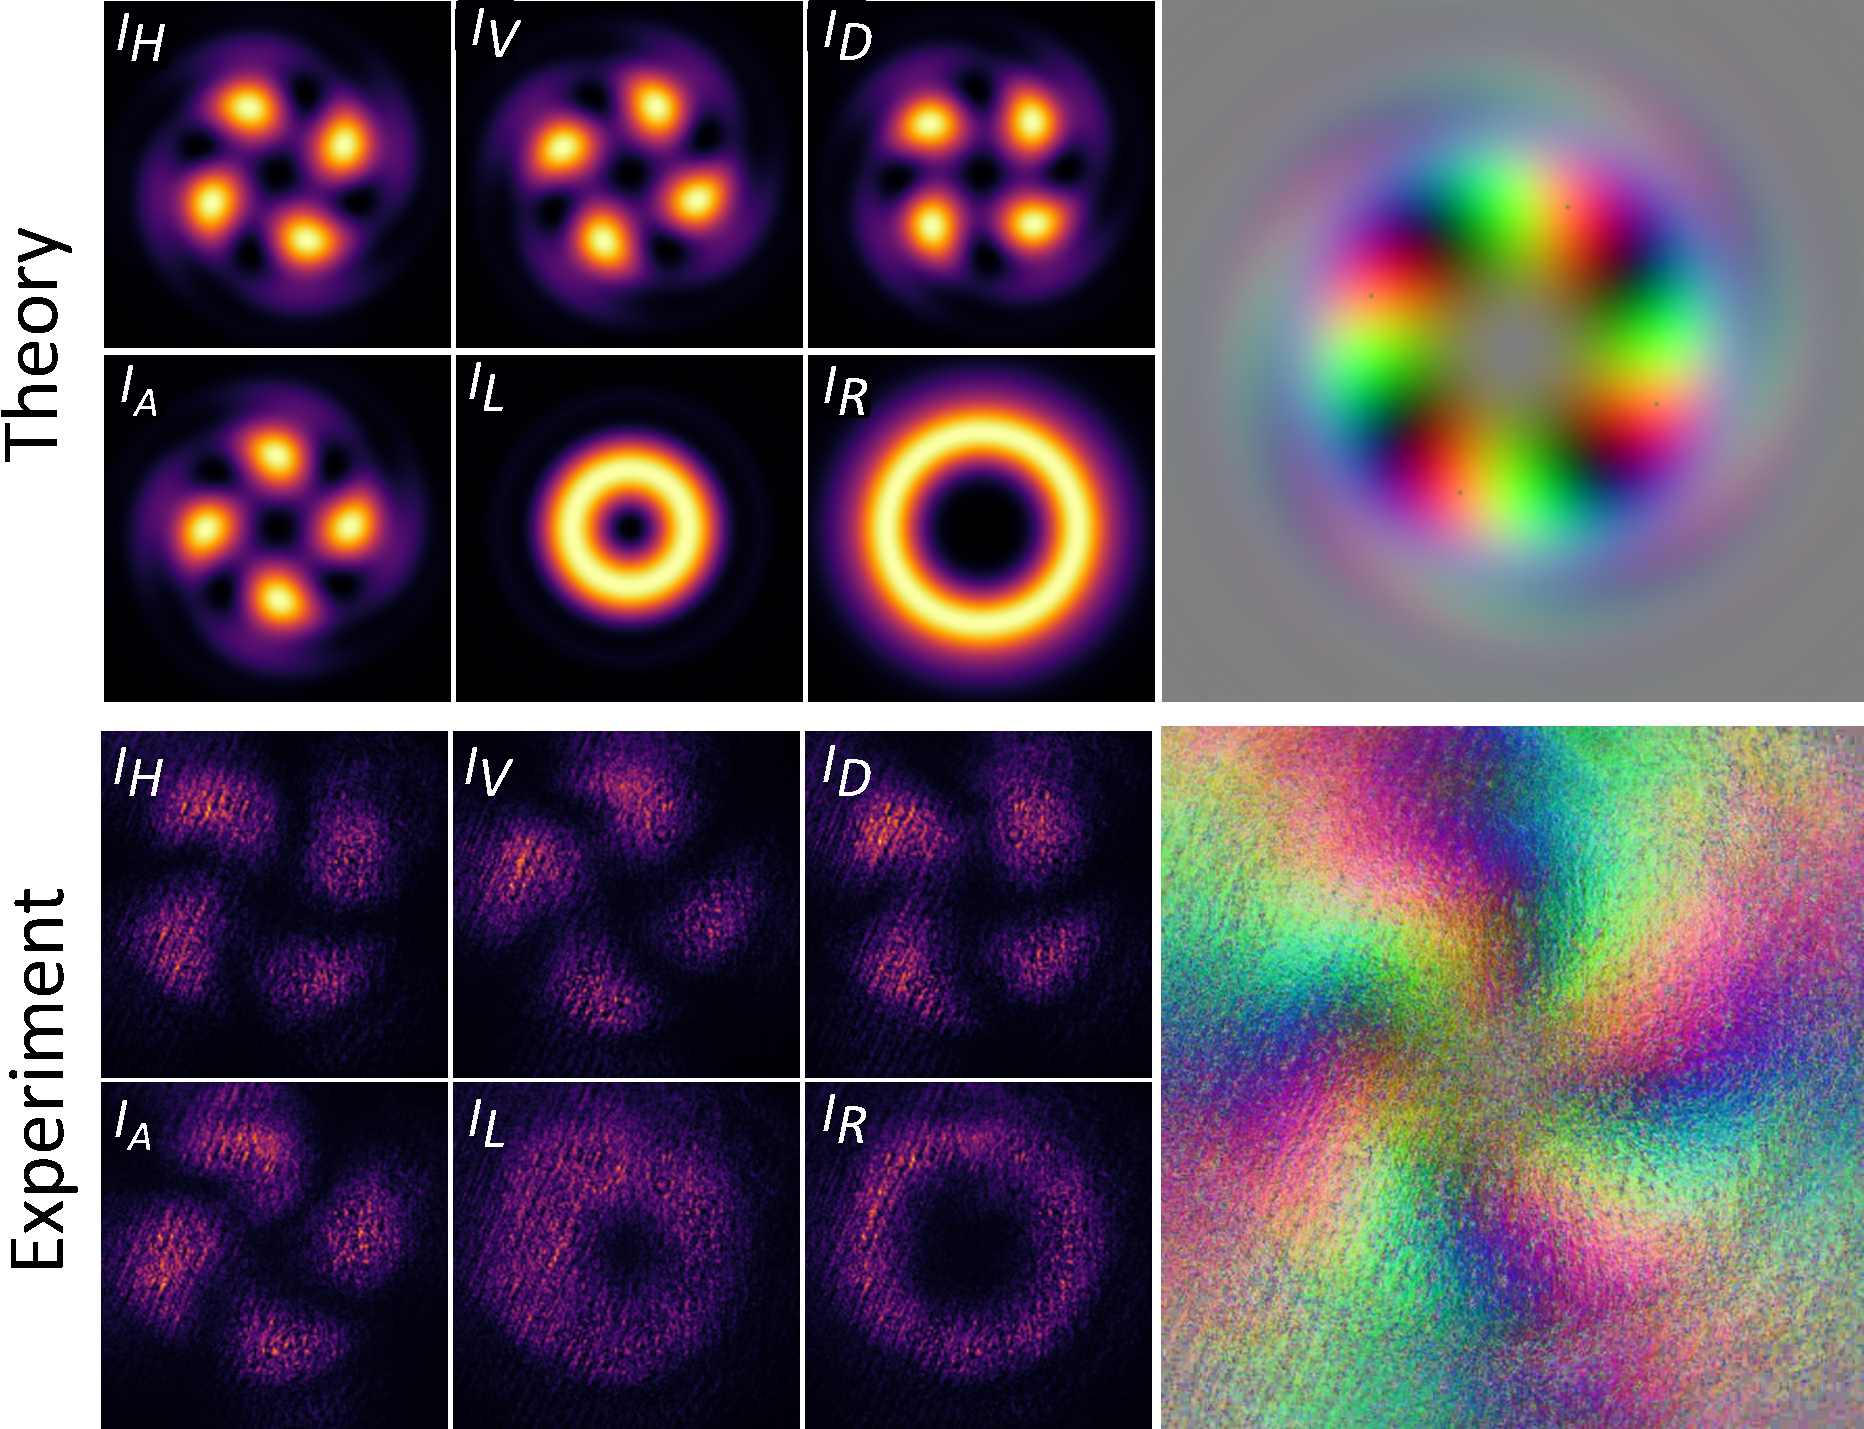
\includegraphics[width=\columnwidth]{supp3.pdf}
    \caption{\textbf{Role of the radial modes.} Simulated images of a VVB generated with HyGG modes. In the calculation we have considered two HyGG modes with $(m_1,m_2)=(-3,1)$ propagating for $z\sim 1\,m$ with a Rayleigh range $z_R\sim 4\,m$. Comparison of the intensities recorded in the polarization measurements in the experiment.}
    \label{fig:my_label}
\end{figure}


The transformation actually operated by a $q$-plate with $q=0.5$ on a LG modes with zero radial number is 
\cite{Karimi:09}
\begin{align}
  \Vec{e}_L \text{ LG}_m &\stackrel{\text{QP}}{\longrightarrow} \Vec{e}_R\,\text{HyGG}_{|m|-|m+1|,m+1}   
\end{align}
The resulting HyGG beam carries OAM equal to $m+1$, but when expressed in the LG basis, it comprises the superposition of several modes with non-zero radial number, namely $\text{HyGG}_{|m|-|m+1|,m+1}=\sum_p c_p \text{LG}_{p,m+1}$. The contributions of the radial modes with $p>0$ can be neglected for $\zeta \ll 1$ and large $m$. For a detailed description of the coefficients $c_p$ see Refs. \cite{Karimi:07,Karimi:09, cardano2015quantum}.

In Fig. \ref{fig:my_label} we report the comparison between the simulated images computed by considering HyGG modes instead of LGs and images recorded in the experiment. The two vortexes in the VVB carry respectively OAM equal to $(m_1,m_2)=(-3,1)$, more precisely we consider a state in the form $ \Vec{e}_R\,\text{HyGG}_{-1,-3}+\Vec{e}_L\,\text{HyGG}_{-1,1}$. The simulation's parameters, such as $\zeta$, were adapted to reproduce the conditions of the experiment.


Even if such simple model of the experimental imperfections seems to be fit for the purpose, it is worth noting that other sources of noise could be investigated. First, in our simple model of the radial-mode contribution via HyGG modes, we did not consider the step-by-step conversion 
operated by the cascaded $q$-plate system in the setup. A more rigorous calculation could take into account the propagation and conversion of the several radial contributions at each step. Other effects in this direction are the non ideal conversion efficiencies: residual lower-$m$ components propagate inside the principal beam and can modify the polarization pattern and the relative weights of the radial modes. In the end, relative misalignment among $q$-plates singularities could affects the quality of the VVBs.


While the inclusion of all such considerations in the calculation of the training set could enhance the performance of a classifier in labelling experimental data, we leave it as a  perspective for a future work. On the other hand, a rigorous model of the imperfections is a complex task and makes the training set tied to the specifics of the experimental apparatus. Consequently, including some experimental images in the training set remains a possible solution.

\section{Classification via CNNs}
\label{sec:CNNs}

We describe here in more details the general structure of CNNs, and how we use them to classify experimental images.
%\replace{CNNs are feed-forward neural networks that find widespread use in the context of ML. They are famous for the outstanding results for visual recognition.
%As all neural network architectures, they are inspired by biological systems in particular by the visual cortex in the brain.}
%\add{%
%\acp{CNN} are a class of feed-forward neural networks that is especially suited to handle images.}
% As all neural network architectures, they are inspired by biological systems in particular by the visual cortex in the brain. (ci serve questa frase?)
%\remove{Their rising success, that coincided with the deep learning renaissance thanks to GPU computational units, was established at the ImageNet Large Scale Visual Recognition Challenge in 2012, which was won by a deep CNN architecture. Nowadays, CNNs have became the leading algorithms for image classification.}
%\highlight{(I don't think this is necessary to add here, but if we do we need to also add the proper citations)}
The typical structure of CNNs is given in Fig.~2a in the main text.
Most CNNs are built as a sequence of three types of layers: convolutional, pooling, and fully-connected layers.
Convolutional layers are used to extract features from the input images. Pooling reduces the number of parameters of the model, cutting down redundant information.
Fully-connected layers are typically used after convolutional and pooling layers, to classify the features extracted by the convolutional layers.
Different CNNs will use different configurations and numbers of these components, depending on the task at hand.

Convolutional layers apply \textit{filters} to the input image. Filters are $k\times k$ matrices which operate by \textit{convolution} on their input. This means that each filter is applied to each pixel $(x, y)$ of its input, and produces the inner product between the elements of the filter matrix and the region neighboring $(x, y)$.
If the input data has different channels (for example different color channels), the filters will have dimensions $n_{ch}\times k\times k$ (\textit{e.g.} $n_{ch}=3$ for RGB images).
Convolutional layers typically use many filters, each extracting different features from the dataset.
For an input image of dimensions $n_{ch}\times N_x\times N_y$, a convolutional layer using $N_c$ filters will thus produce an output with dimensions $N_c\times N_x\times N_y$.
Convolutional layers are followed by a nonlinearity applied elementwise to the outputs.
A common choice for this nonlinearity is the so-called Rectified Linear Unit (ReLU), defined as $x\mapsto\max(x,0)$.
The elements of the filters, as well as the weights connecting the filters to their inputs, are parameters learnt during the training.
% In a standard CNN, The convolution in a particular location $(x,y)$ is obtained by computing the inner product between a $k \times k$ sub region of the input image and a filter of the same size. Repeating this process for each location on the input image, it is possible to obtain an activation map associated to specific features.
Mathematically, we write the output of the $n$-th convolutional layer as
\begin{equation}
    Y_n = \phi(W_n * X),
    \label{eq:ml_conv}
\end{equation}
where $\phi$ is the nonlinear activation function, $X$ the input image, and $W_n$ the set of filters defining the $n$-th convolutional layer, and $*$ represents the convolution operation.
% for the inner product in two dimension, so the convolution between the filter and the image. The activation function is necessary to capture the nonlinear features of the images.
%\rmv{A max-pooling layer is used immediately after the convolutional layer to reduce the number of parameters. The output of the previous layer are then divided into blocks of size $p \times p$, and the $\max$ function is applied over each block.}
% Pooling layers have the role to achieve spatial invariance in features extraction with respect to translation and distortion. This step is crucial for any image recognition protocol.
Pooling layers operate by coarse-graining their inputs.
This is achieved by partitioning the images into windows of size $p\times p$, and mapping each such window into a single numerical output.
Common choices are the so-called \textit{average-pooling} and \textit{max-pooling}, in which each window is mapped into its average and maximum value, respectively.
% The layers basically take the average (average-pooling) or the maximum (max-pooling) value in a small area of size $p\times p$ of the input from the previous layer. In the more recent networks max-pooling is the most employed type of pooling layers. Then after $k$-th pooling, the output will be
More precisely, the elements $Y_{k,ij}$ of the output of a max-pooling layer are connected with its input via
\begin{equation}
    Y_{k,ij} =  \max_{l,m \,\in \,\mathcal{R}_{ij}} X_{k,lm},
    \label{eq:ml_pool}
\end{equation}
where $l,m$ are the locations inside the reception area $\mathcal{R}_{ij}$ and $X_{k,lm}$ is the state of the image after $k$ operations.
Pooling layers are useful in that they allow to extract spatially-invariant features from images, on top of reducing the number of parameters defining the model, thus reducing training times.

Finally, fully connected layers are used to classify the data and determine which features most correlate to a particular output class.
The parameters defining the CNN are typically initialized with random numbers, and then trained using \textit{stochastic gradient descent} optimization~\cite{ruder2016overview}.
For the training, we chose as objective function the \textit{categorical cross-entropy}
$\mathcal{L}=- \sum_{i=1}^{C} x_i\log(\phi(\textbf{x})_i)$, where $x_i$ are the neurons in the final fully-connected layers, $\phi(\cdot)$ the activation function, $C$ the number of classes, and \textit{adam} as type of stochastic gradient descent.
The quality of the classification is quantified by the accuracy $\mathcal A$, defined as the fraction of correctly predicted input images.

To build and train a {CNN} we used the Python library Keras~\cite{chollet2015keras}, with TensorFlow~\cite{tensorflow2015-whitepaper} as backend.
In Fig.~\ref{si_fig:truth_CNN}, we report more in detail the results of the training discussed in Fig.3b in the main text. These were obtained with a CNN composed of three convolutional and max-pooling layers, and two fully connected layers. Each convolutional layer uses $32$ filters of size $3\times3\times3\times$, with ReLU activation function. The pooling layers apply the max operation to blocks of size $2\times2\times3$. Finally, the fully connected layers use the softmax activation function, defined as $\boldsymbol x\mapsto (e^{x_i}/\sum_j e^{x_j})_i$.
% The training phase consisted of a finite number of epochs, each one of which composed of $200$ training steps and $100$ validation steps. (non penso sia necessario menzionare il numero di passi nel training, a meno che non si dia anche il numero preciso di epoche (che comunque non è necessario))

Different CNN architectures were also found to be able to perform the task successfully.
Full details, as well as source code and dataset necessary to reproduce the results of this work, are available in the GitHub repository~\cite{github}.
% \href{https://github.com/lucainnocenti/ML-classification-of-VVBs}{lucainnocenti/ML-classification-of-VVBs}.}
The classification performance can be summarized through a truth-table $\mathcal{T}$ reporting the way in which new images not included in the training set are assigned to different classes. The entries $\mathcal{T}_{ij}={N_{i\rightarrow{j}}}/{N^{tot}_{i}}$ give the number of times $N_{i\rightarrow{j}}$the images labelled by $(m_{1},m_{2})_i$ within the classes reported in Fig.3a of the main text are assigned to the class $(m_{1},m_{2})_j$, divided by the number of images $N^{tot}_{i}$ in the class. %$(m_{1},m_{2})_i$ .} 
%In formula we have $\mathcal{T}_{ij}=\frac{N_{i\rightarrow{j}}}{N^{tot}_{i}}$.}
%We have reported the simple code for generating and training the CNN used in this work above in this section
\begin{figure}[t]
    \centering
    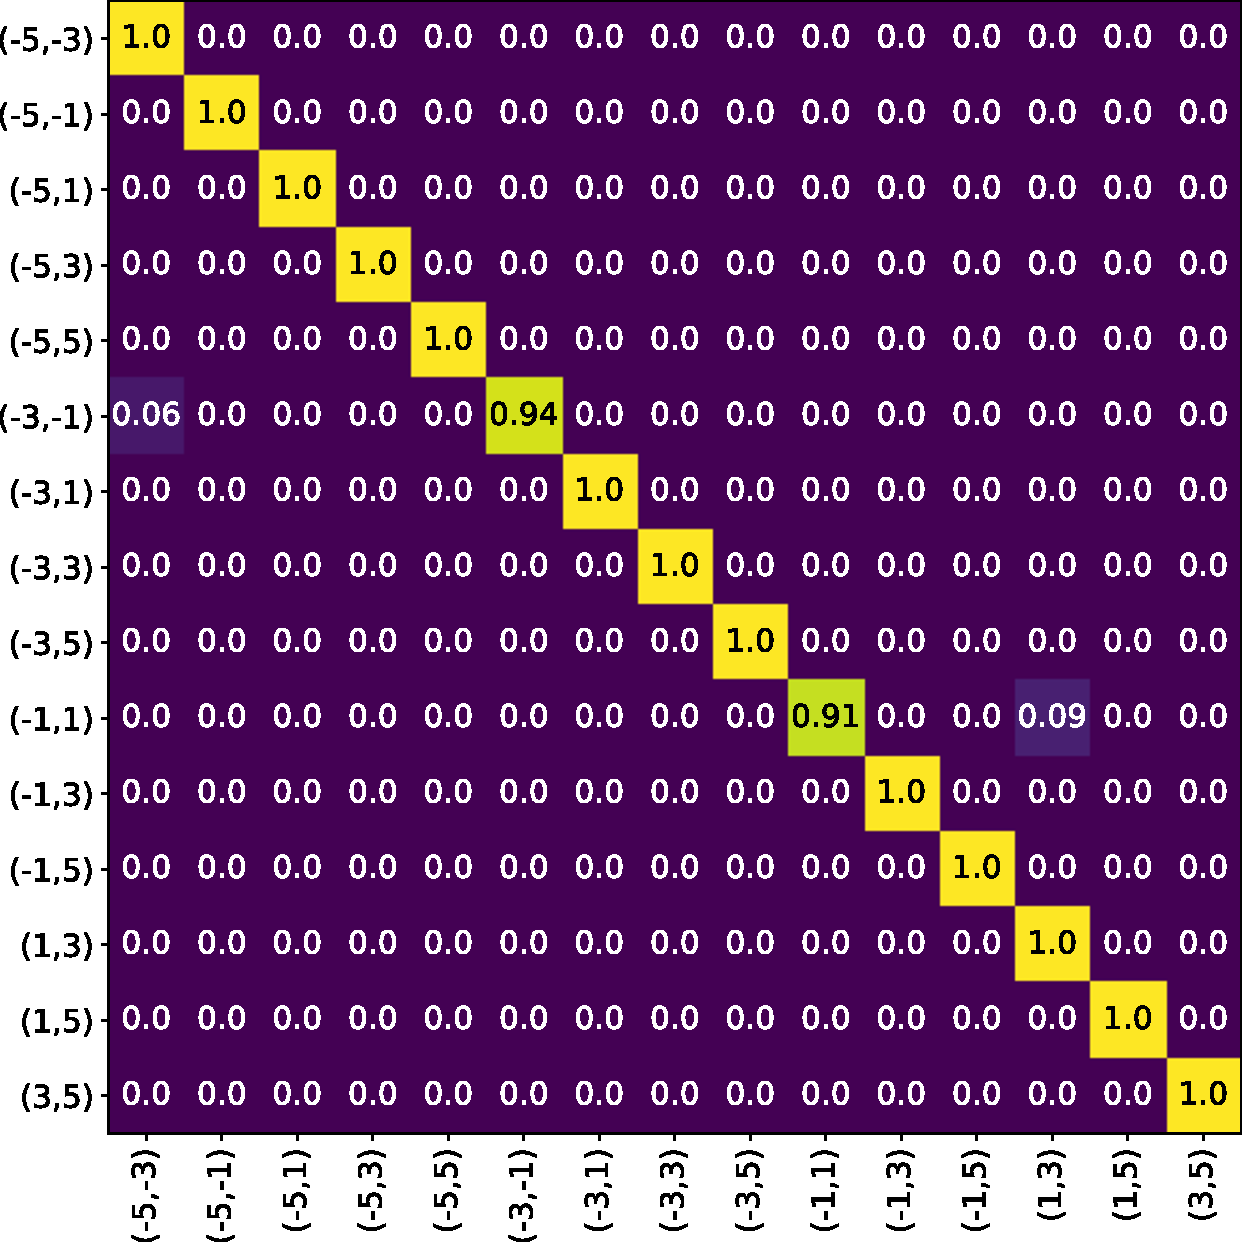
\includegraphics[width=\columnwidth]{truth_table_CNN.pdf}
    \caption{
        \textbf{Prediction accuracies with CNN classifier.}
        A more detailed version of the truth-table given in the inset of Fig.3b in the main text.
        For the $i$-th class (row), we report the fraction of images that are classified by the trained CNN as belonging to the $j$-th class (column).
    }
    \label{si_fig:truth_CNN}
\end{figure}

In Fig.\ref{si_fig:truth_CNN} we report the truth-table displayed in the inset of Fig.3b of the main text. The elements have been computed on a sample of $N_{i}^{tot}=100$ images per each class. %Note that the accuracy defined in eq. \eqref{si_eq:accuracy} can be expressed through the matrix $\mathcal{T}$ noting that $\Bar{N}_{i}=N_{i\rightarrow{i}}$. Then an equivalent definition of accuracy is
%\begin{equation}
%\mathcal{A}=\frac{1}{C}\sum_{i=1}^{C} %\frac{N_{i\rightarrow{i}}}{N^{tot}_i}=\frac{1}{C} \textbf{Tr}\, \mathcal{T}.
%\label{si_eq:accuracy2}
%\end{equation}}
We will use these two quantities $\mathcal{A}$ and $\mathcal{T}$ also to report the classification performance by the Support Vector Machine (SVM).

%\redComm{(unclear)}. 
%\replace{The network training consists of a finite number of epochs each of which composed of $200$ training steps and $100$ validation steps.}{}

\section{Dimensionality reduction}
\label{sec:dimensionality_reduction}

\begin{figure*}[ht!]
    \centering
    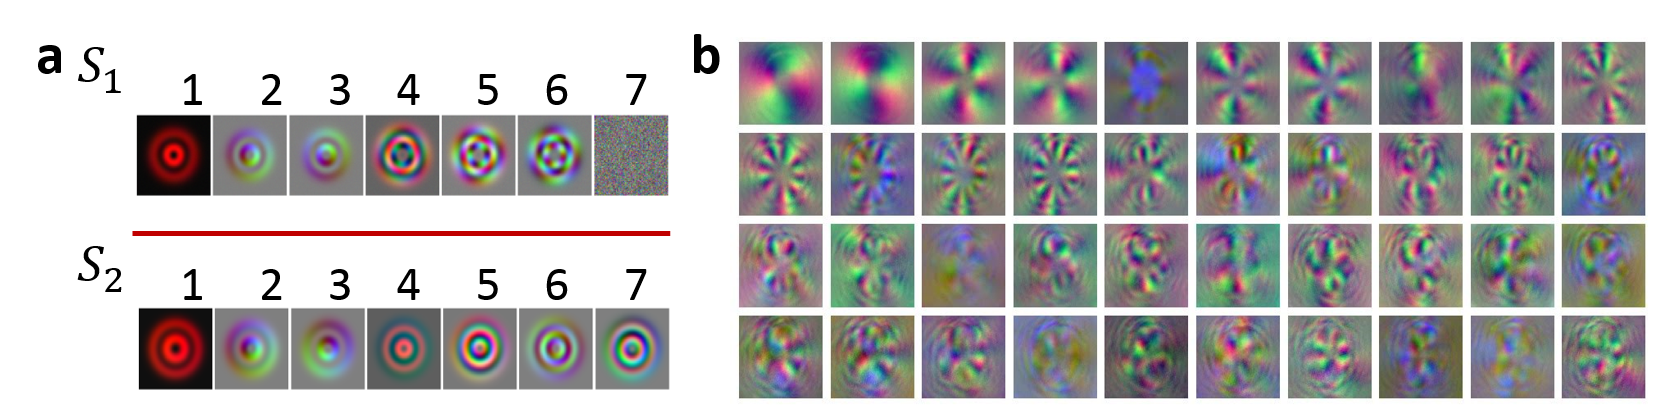
\includegraphics[width=0.98\textwidth]{S1_fig.png}
    \caption{
        \textbf{a,}
        Principal components obtained using PCA on simulated datasets of noisy VVB. The first (second) row shows the first seven principal components obtained on the dataset $\mathcal S_1$ ($\mathcal S_2$). 
        The first 6 (all 7) components correspond to non-vanishing singular values.
        \textbf{b,} First 40 principal components individuated in the experimental dataset corresponding to the 15 classes labelled by $(m_1,m_2)$, discussed in the main text.%
    }
    \label{fig:S1}
\end{figure*}


We discuss here our application of \emph{dimensionality reduction}~\cite{fodor2002survey,cunningham2008dimension} to characterize experimental images.
The main idea of dimensionality reduction algorithms is to reduce the dimensionality of a dataset while retaining as much of its important features as possible.
In particular, we use linear \ac{PCA}~\cite{jolliffe2016principal}.
The goal of \ac{PCA} is to find the directions capturing the maximum amount of information about the dataset. More specifically, if the dataset is comprised of $N$ real vectors of length $M$, defining the \emph{data matrix} $\bs X$ as the $N\times M$ matrix whose $i$-th row is the $i$-th vector, \ac{PCA} finds the vectors $\bs a\in\RR^{M}$ that maximize the variance of $\bs X\bs a$. This turns out to be equivalent to diagonalizing $\bs S\equiv \tilde{\bs X}^T\tilde{\bs X}/(N-1)$, where $\tilde{\bs X}$ is the \emph{centered data matrix}, which is obtained by shifting each column of $\bs X$ so that it averages to zero.
The first $k$ \emph{principal components} found by \ac{PCA} are then the $k$ eigenvectors of $\bs S$ corresponding to the largest $k$ eigenvalues.
Note that these principal components are themselves vectors of the same ``type'' as the data vectors. This means that \ac{PCA} effectively generates a set of data vectors which ``optimally represent'' the information content of the original dataset.

For example, in our case, each row of $\bs X$ is a vector of length $128\times128\times3$ containing the Stokes parameters $S_{b_1}, S_{b_2}, S_{b_3}$ for each pixel of the camera.
Because each image corresponds to such a vector, and vice versa each such vector corresponds to the image of a \ac{VVB}, we can again represent the principal components found by \ac{PCA} as images. This allows to gain intuition into the type of features that optimally represent the data according to \ac{PCA}.

Let now $\rho$ be the density matrix characterizing a \ac{VVB}. The corresponding image is given by the set of real numbers $p_k=(\mathcal U\rho\mathcal U^\dagger)_{kk}$, with $\mathcal U$ the unitary operator performing the basis change from the \ac{OAM} to the position basis. In other words, $\rho$ describes the state in the OAM-polarization basis, which is the basis in which the generated states are efficiently described, whereas $\mathcal U\rho\mathcal U^\dagger$ describes the same state in the position basis, which is the one in which the CCD camera operates.
The set of detected probabilities is then given by
$\bs p=\on{diag}(\mathcal U\rho\mathcal U^\dagger)\equiv\Psi(\rho)$,
where $\Psi$ is the linear map sending $\rho$ to the set of measured probabilities $\bs p$
\footnote{It is worth noting that, while the formalism used in this section is evocative of quantum states being measured in the computational basis, all of the calculations apply equally well when only classical light is used, as is the case in our experiment. A more careful treatment modeling $\rho$ as a multimode coherent states, and $\bs p$ as the set of detected intensities, but give identical results to the ones presented here.}.
% \add{Note that, while we use here a formalism and vocabulary evocative of quantum states, the states actually used in the experiment are classical. This in now way impacts the formal description of the protocol, and the only thing that should change when the states used are classical is that the probabilities $\bs p$ should be reinterpreted as intensities.}
Crucially, the linearity of $\Psi$ implies that it preserves the \emph{convexity} of the space of states, and therefore many of its geometrical features.
For example, if we consider states of the form $c_0 \ket{\uparrow,m=m_1} + c_1 \ket{\downarrow,m=m_2}$ with $m_1\neq m_2$, then the associated density matrices will be arranged to form a three-dimensional sphere embedded in the full state space (because these are effectively different states of a single qubit).
Thanks to the linearity of $\Psi$, \emph{the corresponding probabilities $\bs p$ will also be contained in a spherical surface}, up to possible rescaling of the axes.
In other words, the Bloch sphere of the original two-dimensional system is still present, albeit hidden, in the experimental images, embedded into an extremely high-dimensional space.


To illustrate the usefulness of these ideas in understanding the type of states generated by a given apparatus, we consider here two further examples of applications of \ac{PCA} for different types of input states. 
In all of these cases, \ac{PCA} is applied without any prior knowledge of the input states, and is therefore to be considered a type of \emph{unsupervised learning}.
Consider a simulated set of images corresponding to VVBs of the form
$c_1\ket{L,m=1}+c_2\ket{R,m=2}$ and
$c_1\ket{L,m=1}+c_2\ket{R,m=4}$, where the coefficients $c_i$ are sampled uniformly at random from the set of $c_{1},c_2\in\mathbb{C}$  such that $|c_1|^2+|c_2|^2=1$.
% (\emph{i.e.} uniformly sampled on the Bloch sphere).
Applying PCA to this dataset, we find six non-vanishing singular values, whose associated principal components are given in Fig.~\ref{fig:S1}\textbf{a}.
This is consistent with the dimension of the subspace  spanned by states of the form $\mathcal S_1=\{c_1\ket{L,1}+c_2\ket{R,2}, c_3\ket{L,1}+c_4\ket{R,4}\}$,  as the set of corresponding density matrices is spanned by the six orthogonal matrices
$X^{(1,2)}, X^{(1,4)}, Y^{(1,2)},Y^{(1,4)},Z^{(1,2)}\pm Z^{(1,4)}$, where $X^{(i,j)}=\ketbra{i}{j}+\ketbra{j}{i}$ is the Pauli $X$ matrix acting on the $(i,j)$ subspace, and similarly for $Y^{(i,j)}$ and $Z^{(i,j)}$.
On the other hand, if the dataset under consideration consists of states of the form $\mathcal S_2=\{c_1\ket{L,1}+c_2\ket{R,2}, c_3\ket{L,3}+c_4\ket{R,4}\}$, then \ac{PCA} finds \emph{seven} principal components associated with non-vanishing singular values (see Fig.~\ref{fig:S1}\textbf{a}).
This is consistent with the underlying state space being spanned by the seven orthogonal Hermitians:
\begin{equation}
\begin{gathered}
    X^{(1,2)}, \,\, X^{(3,4)}, \,\,
    Y^{(1,2)}, \,\, Y^{(3,4)}, \\
    Z^{(1,2)},\quad
    -Z^{(1,2)} + 2 Z^{(1,3)}, \\
    -Z^{(1,2)} - Z^{(1,3)} + 3 Z^{(1,4)}.
\end{gathered}
\end{equation}
These matrices can be obtained by direct analysis of the type of states contained in $\mathcal S_2$ and then finding a set of orthogonal Hermitian matrices generating the corresponding set of density matrices.
It is worth noting how this method provides a quick and easy way to gain useful information about the dimensionality of generated states, as well as about other properties such as specific symmetries, which, as shown in~\cref{fig:S1}, are often picked up by the principal components.


\section{Support vector machines}
\label{sec:SVMs}

\begin{figure}[t]
    \centering
    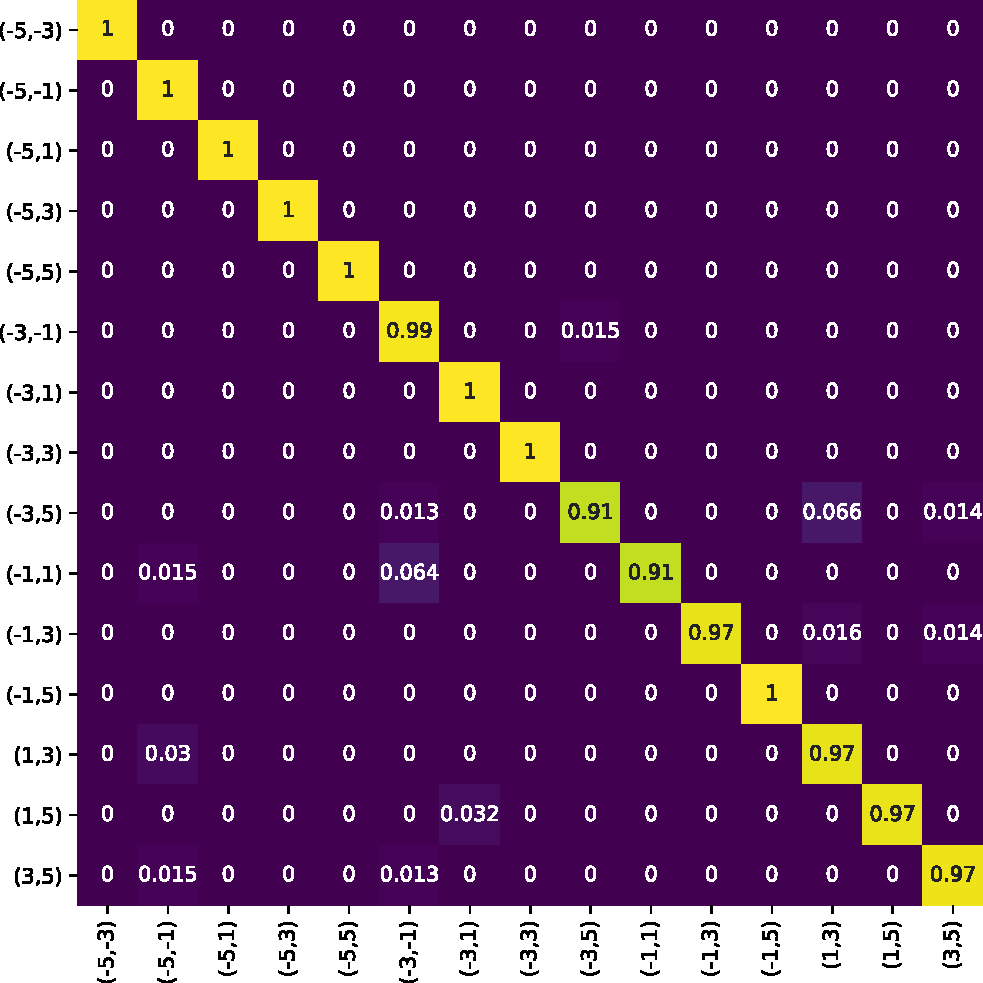
\includegraphics[width=\columnwidth]{truth_table_PCA+SVC.pdf}
    \caption{
        \textbf{Prediction accuracies with SVC classifier.}
        Each row and column corresponds to a different class.
        The $i$-th row gives the number of images predicted (correctly or not) by the classifier as belonging to the $j$-th class, for each $j$.
    }
    \label{si_fig:truth_SVC}
\end{figure}

Once \ac{PCA} has been used to find reduced representations for the experimental images, simple classification methods such as \acp{SVM}~\cite{hearst1998support,shawe2000support} can be used to categorize them.
We use here in particular a \emph{linear}, multiclass \ac{SVM}, whose goal is to find hyperplanes in the feature space that optimally separate the datapoints corresponding to different classes.
During the training phase, a set of training experimental images is used to find the separating hyperplanes, which can then be used to classify new experimental images.

We train a \ac{SVM} on the reduced $40$-dimensional representation found via \ac{PCA} (the corresponding principal components are shown in Fig.~\ref{fig:S1}\textbf{b}). The goal is, similarly to what we did with the \ac{CNN}, to categorize experimentally generated \acp{VVB} in one of the $15$ classes characterized by their OAM quantum numbers $(m_1,m_2)$.
% In our work a linear support vector machine (SVM) has been employed for this task. Support vector machines are very well-known linear classifiers in machine learning. The algorithm is fed with a series of labelled data during the training stage as to retrieve the optimal hyperplane which separates the elements of different classes. In the present case the SVM finds the optimal separation between experimental images of the training set expressed in the reduced space, described by the principal components in Fig. \ref{fig:S1}b.
This results in an average classification accuracy of $\sim 98 \%$.
A more detailed breakdown of the results of the classifier is given in Fig.~\ref{si_fig:truth_SVC}.
This result confirms that the compressed representation found via \ac{PCA} is sufficient to capture the important features of the generated states, thus allowing for more efficient classification schemes.


\bibliography{vvb}
\bibliographystyle{apsrev4-1}
\end{document}
